% ###################################################################
% #  GENERATED FILE -- DO NOT EDIT.                                 #
% #                                                                 #
% #  Assembled by build.py from _head.tex + _body.tex + _tail.tex.  #
% #  Any edit here is silently overwritten on the next build.       #
% #  Edit the fragments instead, then run:  python build.py         #
% ###################################################################

% =====================================================================
%  Below the Noise Floor
%  GLEE Competition paper -- IAB Workshop, NeurIPS 2026
%  Agent ID: 7aidara_Gamma  (agent track, 6th place)
%
%  BUILD
%    Put the official neurips_2026.sty beside this file, then
%      pdflatex glee_competition_paper   (twice)
%    Without it the preamble falls back to a geometry-matched article
%    class (5.5in x 9.0in text block) so the draft still compiles.
%
%  PAGE LIMIT
%    Main body = pages 1-4, ending at \section{Conclusion}.
%    References are unlimited. Everything after \appendix is
%    SUPPLEMENTARY -- delete it if the chairs enforce "references only".
% =====================================================================
\documentclass{article}

% `preprint` = non-anonymous (the competition track is single-blind) without the
% camera-ready footer that `final` would print, since this is a workshop
% competition-track submission and not a NeurIPS main-conference paper.
\IfFileExists{neurips_2026.sty}{%
  \usepackage[preprint]{neurips_2026}%
}{%
  % Same 5.5in x 9.0in text block, so a draft still paginates faithfully if the
  % official style file is missing.
  \usepackage[letterpaper,margin=1.5in,top=1.0in,bottom=1.0in]{geometry}
  \usepackage{times}
  \typeout{*** neurips_2026.sty not found -- fallback geometry in use ***}
}

\usepackage[utf8]{inputenc}
\usepackage[T1]{fontenc}
\usepackage{hyperref}
\usepackage{url}
\usepackage{booktabs}
\usepackage{amsfonts}
\usepackage{amsmath}
\usepackage{microtype}
\usepackage{xcolor}
\usepackage{tikz}
\usepackage{float}

\newcommand{\tbf}[1]{\textbf{#1}}
\newcommand{\tsm}[1]{\texttt{\small #1}}

% --- styles used by fig_noise.tex ------------------------------------
\definecolor{c1c}{HTML}{2F6F8F}
\definecolor{c2c}{HTML}{C2632B}
\definecolor{c3c}{HTML}{6C8B3C}
\definecolor{c4c}{HTML}{8B5E9C}
\definecolor{c5c}{HTML}{B03A48}
\definecolor{inkc}{HTML}{3A3A3A}
\tikzset{
  gridline/.style={draw=black!12,line width=0.35pt},
  axline/.style={draw=black!45,line width=0.5pt},
  axlab/.style={font=\scriptsize,text=black!60},
  ptlab/.style={font=\scriptsize\bfseries},
  note/.style={font=\scriptsize,text=inkc,inner sep=1pt},
  band/.style={fill=black!7},
  spreadarrow/.style={draw=inkc,line width=0.7pt,|<->|,>=stealth},
  c1/.style={draw=c1c}, c2/.style={draw=c2c}, c3/.style={draw=c3c},
  c4/.style={draw=c4c}, c5/.style={draw=c5c},
}

\title{Below the Noise Floor: A Deterministic GLEE Agent\\
       and the Measurement Problem It Exposed}

\author{%
  Yosef Zoabi\\
  \texttt{yosef.zoabi@campus.technion.ac.il}\\
  \texttt{\small GLEE Agent ID \texttt{edb1db91303e} (7aidara\_Gamma)}\\
  \texttt{\small Agent track: 6th place. Human track: \textbf{2nd place}.}
}

\begin{document}
\maketitle

\begin{abstract}
I competed in both GLEE tracks: as \textsc{7aidara\_Gamma}, a deterministic,
LLM-free agent that finished \tbf{6th in the agent track} (2360.8) over
\tbf{264{,}432 games and 3.11M logged turns}, and by hand, where I finished
\tbf{2nd in the human track}. The agent is ${\approx}2{,}300$ lines of
Python, one closed-form policy per family behind 114 parameters, with no learning
and no language model. My central finding is methodological and negative:
\tbf{GLEE's percentile-Elo cannot resolve the effects entrants are trying to
produce}. Five \emph{byte-identical} builds, polled simultaneously for 8.6 hours
over ${\approx}3{,}000$ games each, differed by up to 88 rating points overall and
293 within a family, while their \emph{behaviour} differed by ${\le}0.010$ of the
pot; separating two policies that differ by 0.25 rating points per game at
$3\sigma$ needs ${\approx}5{,}600$--$6{,}700$ games \emph{per arm}. Across 30+
interventions and 49 runs only \emph{strictly dominated} fixes ever replicated,
every tuning arm measured nothing, and one unmeasured arm shipped fleet-wide cost
100--385 negotiation points per agent. Much of what the policies rely on is not
documented anywhere and had to be recovered from play: the valuation pool, an
undisclosed round cap that pays both sides nothing, and the rating's own update
rule. I give four offline techniques that measured what the leaderboard could
not, a survivorship failure mode that silently corrupted four analyses, and a
measurement of what abandoning games actually costs. Playing both tracks yields
an unusually controlled human-versus-machine comparison, one designer and one
shared opponent pool, which finds that agent and human read seller messages
equally well (hit rate 0.738 vs.\ 0.725) and separate almost entirely on the
discipline to decline.
\end{abstract}

\section{Introduction}

GLEE~\cite{shapira2024glee}, in the lineage of automated negotiation
competitions~\cite{anac2011,baarslag2014decoupling}, evaluates agents in three economic
families: \emph{bargaining} (alternating-offer division with discounting),
\emph{negotiation} (bilateral trade under private valuations~\cite{myerson1983}) and
\emph{persuasion} (a 20-round sender--receiver game). Configurations come from a
grid of 960 combinations, and payoff is scored not in dollars but as a
\emph{percentile} against every payoff earned on the same configuration in the
same role, adjusted for opponent strength:
$r_{\text{game}} {=} 2000 + 8000(\text{pct}{-}0.5)$,
$\Delta R {=} \eta(r_{\text{game}}{-}R)$, $\eta \to 0.002$.

Two consequences shaped every decision. A \$0 no-deal sits at the bottom of that
scale, so closing a mediocre deal strictly dominates holding out and missing. And
the step size I recovered from my own rating deltas, $\eta{=}0.002$, implies an
EMA half-life of ${\approx}346$ games \emph{per family}: the rating is a smoothed,
lagged, opponent-contaminated statistic, and it is the only feedback the platform
gives.

I built a deterministic agent rather than an LLM one for three reasons. Percentile
scoring over a known parametric family rewards a correct decision rule; the
free-text channel measured as inert (\S\ref{sec:ledger}); and determinism buys
what mattered most, namely that \tbf{a logged game replays to exactly the same
decisions}, which made offline evaluation possible once I found that the
leaderboard could not evaluate anything.

One theme runs through what follows: \tbf{most of what the agent exploits is
undocumented and had to be inferred from play}, so every such fact is stated with
the evidence that recovered it. The paper also spans the workshop's three levels:
what the agent did (\S\ref{sec:aba}), what I did facing the same games by hand
(\S\ref{sec:human}), and where the two diverge. I contribute the agent
(\S\ref{sec:agent}), a measurement of the competition's evaluation noise floor and
the sample it implies (\S\ref{sec:noise}), four offline techniques that measure
strategy changes without the leaderboard (\S\ref{sec:measure}), a ledger of what
replicated and what cost me places (\S\ref{sec:ledger}), the required behaviour
analysis (\S\ref{sec:aba}), and a same-author human baseline (\S\ref{sec:human}).
\section{The agent, and what had to be discovered to build it}
\label{sec:agent}

A dispatcher routes each game by family to one of three closed-form
policies\footnote{\tbf{LLM usage.} The agent contains no language model. I used an
LLM coding assistant for analysis scripts and drafting under my direction, and
verified every reported number against the logs.} (858 / 660 / 781
lines), set by 114 tunables and covered by 472 behavioural tests. Any policy that
raises is replaced by a legal fallback: abandonment scores at the \tbf{5th
percentile} and three self-timeouts trigger a 30-minute queue ban, so a crashing
policy is far worse than a mediocre one. No game in 264{,}432 was lost to an
exception.

\tbf{Bargaining} anchors on the infinite-horizon fixed point
$(1{-}\delta_{\text{them}})/(1{-}\delta_{\text{us}}\delta_{\text{them}})$~\cite{rubinstein1982}
rather than the finite recursion, which swings between ${\approx}0.24$ and
${\approx}0.91$ with the horizon's \emph{parity} and is right only against an
opponent playing the same equilibrium: the agent banks 0.364 where it says 0.236.
Parity still buys a \emph{guarantee}, since if the last proposal is mine the agent
can refuse everything and reach it, priced at what that seat empirically returns
(91.9\% signed, $n{=}1{,}415$). It never walks away, since that pays what running
out of rounds pays.

\tbf{Negotiation} rests on a fact the documentation does not state. Sorting every
valuation the server dealt me showed they are not continuous but drawn from three
fixed four-rung pools, $(80,100,120,150)$ scaled by $\{1,10^2,10^4\}$, both
players on the same scale. My own value therefore pins the whole ladder, so the
agent prices at \emph{tradable rungs} walked from the top down instead of guessing
a reservation price. Roles are drawn independently of values, so only 37.5\% of
hidden-value games hold any surplus and a seat with none is walked at once.

\tbf{Persuasion} rests on a second undocumented fact, verified over 1{,}829 sold
rounds: the seller is paid the full price on \emph{every} sale, high or low, so
reputation is the only currency. Bayesian persuasion~\cite{kamenica2011bayesian}
then fixes the tolerable lie rate: recommending every high unit and a fraction $q$
of low ones puts the buyer's posterior at $p/(p{+}(1{-}p)q)$, so
$q^\star{=}p(1{-}\tau)/(\tau(1{-}p))$ for threshold $\tau$. The agent spends under
it, ramping as rounds run out (Appendix Table~\ref{tab:ladder}). A
third undocumented fact, found from a cluster of \$0 outcomes at high round
numbers, reshaped both open-horizon policies: games sold as unlimited stop at a
round cap paying \emph{both} sides nothing.

\section{The measurement problem}
\label{sec:noise}

Because only an account's \emph{best} agent is ranked, my five slots could be
spent as five simultaneous \emph{controls} rather than five experiments
(Appendix Table~\ref{tab:volume}), which turns an unfalsifiable rating into a
measured null. Polled together for 8.6 hours over ${\approx}3{,}000$ games each,
five \tbf{byte-identical} builds spread a mean of 48.1 rating points and up to
292.9 within a family, while their \emph{behaviour} differed by ${\le}0.010$ of
the pot (Appendix Figure~\ref{fig:noise}).

\tbf{The size of that noise is arithmetic.} The rating is an 80-fold
magnification of a percentile, so with $\eta$ decayed the displayed rating inverts
to $\mathrm{pct}{=}0.5+(R{-}2000)/8000$, evaluated where the field's payoff
density is highest. A 346-point bargaining collapse was a move from the 51.8th
percentile to the 47.4th, and the final board is compressed the same way:
\tbf{ranks 3 to 7 of the agent track are separated by 0.41 percentile points},
and the 10.5 rating points by which I missed 5th are 0.13 of one.
Appendix~\ref{app:scoring} has three further properties of the rule.

Two further properties compound it. The pool is \tbf{non-stationary}, since
scoring is against the research dataset \emph{plus competition games as they are
played}, so \emph{no cross-time comparison is valid}; and ratings \tbf{freeze when
idle}, making the close a stopping problem. I banked $+83$ points by freezing an
agent on a one-hour high, and on the final evening three of the four accounts
above me had already stopped playing. Worse, \tbf{almost every run is
underpowered}: the per-game rating delta has $\mathrm{sd}{=}4.84/4.42/4.44$ over
120{,}023 games, so separating two arms differing by $\Delta$ at $3\sigma$ needs
$n{=}(3\sigma\sqrt2/\Delta)^2$ games \emph{each}, or \tbf{6{,}743 / 5{,}632 /
5{,}689 per arm at $\Delta{=}0.25$}, against effects of 0.05--0.20 and a best
window of ${\approx}4{,}000$ games per agent.

\section{Measuring without the leaderboard}
\label{sec:measure}

Four offline techniques carried essentially all my evidence, using only my own
logs; the fourth, which recovers the quality rate on \emph{declined} rounds by
subtraction from the known prior, is in Appendix~\ref{app:lim}.

\tbf{(A) Paired within-game counterfactuals.} Accepting is \emph{unilateral and
terminal}, so the other branch is arithmetic: signing now is exactly
$\text{share}\times\delta^{(r-1)}$, which makes every refused offer its own
control, with no survivorship. It gave a break-even accept bar per configuration
from 23{,}617 refusals.

\tbf{(B) Decision-level replay, as a mandatory pre-flight.} The turn logs re-run
the shipped decision function exactly, reproducing \tbf{4{,}272 of 4{,}272}
bargaining and \tbf{13{,}056 of 13{,}056} negotiation decisions with zero
mismatches, so the replay \emph{is} the agent. Count the decisions a
flag \emph{changes}, which is \emph{not} how often its condition fires: one arm's
condition held on 43\% of eligible games and changed \tbf{0 of 13{,}056}
decisions, another \tbf{0 of 13{,}479}.

\tbf{(C) Break-even recovery.} $\Delta R$ is monotone in percentile, so the
outcome at which mean $\Delta R$ crosses zero is the outcome ranking at my own
standing, the field median when $R{\approx}2000$. Fitting $\Delta R$ on banked
share within a configuration and taking the root uses \emph{every} game, \$0
no-deals included, so there is no survivorship (slope positive in 58 of 64 cells,
median $R^2{=}0.60$, split-half $r{=}0.741$). It localised my bargaining deficit
to a single seat, and showed the loss there was the accept
bar~\cite{baarslag2013acceptance}, not the opening ask. Across all 55 cells
it also characterises the field: its median tracks Rubinstein SPE where that
prediction is interior ($r{=}0.895$, mean gap 0.070 of pot) and abandons it where
it is extreme (gap 0.281), taking \tbf{0.297} where theory says take nothing and
\tbf{0.734} where it says take everything~\cite{ochsroth1989}. An equilibrium
anchor is therefore miscalibrated at the grid's edges
(Appendix Tables~\ref{tab:breakeven} and~\ref{tab:spe}).

\tbf{The failure mode these replace.} Four analyses were wrong the same way:
\tbf{the filter that built the sample already excluded every game that would have
contradicted it} (Appendix~\ref{app:simpson}).

\section{What worked, what failed, and what it cost}
\label{sec:ledger}


Six changes replicated, each removing a \emph{strictly dominated} choice, an
option plainly worse than an available alternative (Appendix Table~\ref{tab:ledger}).

\tbf{Nothing else replicated.} Seven consecutive tuning arms landed inside the
noise floor, as did a seller lie-rate arm held at 100\% against 40\% controls
across three runs ($t{=}{-}0.29$). \tbf{The most expensive mistake was mine}: on
the final morning I shipped one negotiation concession parameter to \emph{all
four} unfrozen agents at once and left it five hours before measuring. It cost
\tbf{100--385 negotiation points per agent}, and I finished 10.5 points behind
5th; one retained control would have caught it in an hour.

\tbf{Abandoning games costs less than it appears to.} An abandoned game scores at
the 5th percentile, and stopping a run kills what is in flight: I abandoned
\tbf{80 of 109{,}881} rated games (0.073\%), 78 of them inside seven clock hours,
at $-6.76$ rating points against $+0.17$ for a game played out. The steps sum to
$-541$, but the rating is an EMA, so the persistent shift is about \tbf{0.5
points}; the close is the exception, where nothing is averaged away.

\tbf{My two best changes came from reading transcripts, not aggregates.} One is a
parser bug: purchases made against messages saying, in plain English, ``\emph{Not
this one\dots pass this round.}'' The refusal list held \tsm{"not this round"} but
not \tsm{"not this one"}, and such near-misses fell through a default branch that
read anything unmatched as a recommendation. Re-scoring 123{,}700 buyer rounds,
270 of the re-classified rounds were purchases and \tbf{258 of them were low
quality}. The other was a 96-round stall showing that my acceptance gate opened at
round 97 in games the server killed at 96. A third reading settled the
architecture: \tbf{language was inert}, the free-text channel moving buyer take-up
only from 0.689 to 0.693~\cite{crawford1982strategic}.

\section{Agent Behavior Analysis}
\label{sec:aba}

\paragraph{What the agent actually did.} Bargaining settled at median round 2 with
a 1.5\% no-deal rate, banking 0.429 of the pot. Negotiation correctly walked
79.8\% of untradable seats, and agreed 20--24\% under hidden values against
85--89\% under complete information. The persuasion buyer shows the intended
discontinuity: 17.4 purchases per game where buying blind pays, 2.2 where it does
not, and the patient-hold gate fires on \tbf{60.7\%} of player-1
$\delta{=}0.95$ decisions against \tbf{0.0\%} of player-2 $\delta{=}1.0$.

\paragraph{How alignment is enforced.} The 472 tests assert the decision the
policy must make in a named regime rather than a utility: at HEAD all pass, while
the final night's working tree, still carrying that run's arm flags, fails 27,
each naming the behaviour its flag changed. Randomisation is seeded from
\tsm{(game\_id, round)}, so the agent is a pure function of observed state, and
technique (B) reproduces 100\% of 17{,}328 logged decision points.

\paragraph{Four cases where it did \emph{not} match design.} \tbf{(1) Rules that
could never fire}: three flags changed zero decisions or were unreachable, so
intent and behaviour were different things. \tbf{(2) A safety valve keyed to the
wrong horizon}: my accept collapse armed two rounds from a cap recorded as 99, in
a family whose games died at 96, so it never fired and 78.8\% of open negotiations
ended at \$0. \tbf{(3) A parser whose default was the wrong way round}, which made
the failure silent. \tbf{(4) A schedule that met its target and lost anyway}: 86\%
of games ground to the last round and dumped for \emph{any} positive profit at
$-6.4$ rating per game, which deal rate could not see because the capitulation
\emph{is} a deal (Appendix Table~\ref{tab:endgame}).

\section{A same-author human baseline}
\label{sec:human}

\begin{table}[htbp]
\centering\footnotesize
\caption{Human versus agent on identical configurations. Bargaining: mean banked
share, known horizon. Persuasion: buyer seat, by whether buying \emph{blind} pays.}
\label{tab:human}
\begin{tabular}{@{}lrrr@{\hspace{1.5em}}lrrr@{}}
\toprule
\multicolumn{4}{@{}c}{\tbf{Bargaining (known horizon)}} &
\multicolumn{4}{c@{}}{\tbf{Persuasion (buyer seat)}} \\
\cmidrule(r{1.5em}){1-4} \cmidrule(l){5-8}
seat & cells & human & agent & regime & human & agent & $t$ \\
\midrule
player 1 (first mover) & 14 & 0.444 & 0.447 & $mp{>}1$ (blind gain) & $+24.22$ & $+22.10$ & $+1.31$ \\
player 2 (last word) & 13 & 0.512 & \tbf{0.720} & $mp{=}1$ (knife edge) & $+2.99$ & $+2.56$ & $+0.56$ \\
 & & & & $mp{<}1$ (blind loss) & $-0.61$ & \tbf{$+0.18$} & $-2.44$ \\
\bottomrule
\end{tabular}
\end{table}

I also played the \emph{human} track by hand and finished \tbf{2nd} over 2{,}690
rated games against the same pool. Reconstructed from per-game deltas my ratings
were 2437\,/\,2406\,/\,2170 against the agent's 2128\,/\,2818\,/\,2136; since the
tracks rank separately I rest the analysis on \emph{matched configurations}
(Table~\ref{tab:human}).

\tbf{(1) Agent and human read sellers equally well}: hit rate on purchases 0.738
over 2{,}745 for me, 0.725 over 59{,}603 for the agent, so the intuition that a
person reads deception better than a keyword list is unsupported. \tbf{(2) The
machine's edge is patience, and the seat it unlocks}: holding the final proposal
it banks 0.720 of the pot against my 0.512, and refusing was correct in
\tbf{96.5\%} of its 13{,}180 measurable games against \tbf{70.4\%} of my 455. In
the first-mover seat the two are level. \tbf{(3) My cost is discipline, not
perception}: where participation does not pay I still buy 8.4 units per game in
cells the agent declines ($t{=}{-}2.44$), and banking zero costs only $-0.04$ to
$-3.15$ points where a \emph{negative} payoff costs $-4.96$ to $-7.65$.

\section{Limitations, reproducibility, and conclusion}

Every number here is confounded by a non-stationary pool and by one account in one
competition; technique (C) assumes $\Delta R$ is locally linear; and the human
sample is one person. The largest gap is \tbf{cross-game
memory}~\cite{baarslag2016survey}: honesty profiles are stable (split-half
$r{=}0.786$) but exploiting them needs state the architecture lacks
(Appendix~\ref{app:lim}). Much of the edge came from undocumented facts recovered
from my own logs, a reproducibility hazard as much as an advantage; the agent
itself is reproducible, being three modules, one parameter file, 472 offline
tests, and every turn logged. Four lessons remain: \tbf{measure your noise floor
first}; \tbf{prefer strictly dominated fixes}; \tbf{replay before you run};
\tbf{read transcripts}. A leaderboard is a scoreboard, not an instrument.

\phantomsection\label{END}
\bibliographystyle{plain}
\begin{thebibliography}{99}\small

\bibitem{shapira2024glee}
E.~Shapira, O.~Madmon, M.~Tennenholtz, and R.~Reichart.
GLEE: A unified framework and benchmark for language-based economic environments.
\emph{arXiv:2410.05254}, 2024. \url{https://arxiv.org/abs/2410.05254}

\bibitem{rubinstein1982}
A.~Rubinstein. Perfect equilibrium in a bargaining model.
\emph{Econometrica}, 50(1):97--109, 1982.

\bibitem{kamenica2011bayesian}
E.~Kamenica and M.~Gentzkow. Bayesian persuasion.
\emph{American Economic Review}, 101(6):2590--2615, 2011.

\bibitem{crawford1982strategic}
V.~P. Crawford and J.~Sobel. Strategic information transmission.
\emph{Econometrica}, 50(6):1431--1451, 1982.

\bibitem{myerson1983}
R.~B. Myerson and M.~A. Satterthwaite. Efficient mechanisms for bilateral trading.
\emph{Journal of Economic Theory}, 29(2):265--281, 1983.

\bibitem{baarslag2014decoupling}
T.~Baarslag, K.~Hindriks, M.~Hendrikx, A.~Dirkzwager, and C.~Jonker.
Decoupling negotiating agents to explore the space of negotiation strategies.
In \emph{Novel Insights in Agent-based Complex Automated Negotiation}, 2014.

\bibitem{baarslag2013acceptance}
T.~Baarslag, K.~Hindriks, and C.~Jonker. Acceptance conditions in automated negotiation.
In \emph{Complex Automated Negotiations}, 2013.

\bibitem{baarslag2016survey}
T.~Baarslag, M.~J.~C. Hendrikx, K.~V. Hindriks, and C.~M. Jonker.
Learning about the opponent in automated bilateral negotiation: a comprehensive
survey of opponent modeling techniques.
\emph{Autonomous Agents and Multi-Agent Systems}, 30(5):849--898, 2016.

\bibitem{anac2011}
T.~Baarslag et al. Evaluating practical negotiating agents: results and analysis
of the 2011 international competition.
\emph{Artificial Intelligence}, 198:73--103, 2013.

\bibitem{ochsroth1989}
J.~Ochs and A.~E. Roth. An experimental study of sequential bargaining.
\emph{American Economic Review}, 79(3):355--384, 1989.

\end{thebibliography}

% =====================================================================
%  SUPPLEMENTARY MATERIAL -- not part of the 4-page main body.
% =====================================================================
\appendix
\newpage
\section{Supplementary figure and tables}

% Appendix floats are numbered A1, A2, ... so a reference from the main text
% reads unambiguously as supplementary material.
\setcounter{table}{0}
\setcounter{figure}{0}
\renewcommand{\thetable}{A\arabic{table}}
\renewcommand{\thefigure}{A\arabic{figure}}

\begin{table}[H]
\centering\small
\caption{Seller-script ladder (persuasion buyer seat): forward hit rate on the
\emph{next} purchase, conditioned on what that exact message template has
already delivered earlier in the same game (6{,}185 buyer replays). The 5.3\%
row sits below the break-even bar $1/m$ in every cell, which is what makes the
template veto strictly dominated.}
\label{tab:ladder}
\begin{tabular}{@{}lrlr@{}}
\toprule
Prior record of this template & hit rate & Prior record & hit rate \\
\midrule
no prior           & 70.4\% & all-low $\times1$ & 33.8\% \\
all-high $\times1$ & 81.3\% & all-low $\times2$ & 19.3\% \\
all-high $\times2$ & 84.8\% & all-low $\times3$ & \tbf{5.3\%} \\
all-high $\times3$ & 91.2\% & mixed             & 63.7\% \\
\bottomrule
\end{tabular}
\end{table}

\begin{figure}[H]
\centering
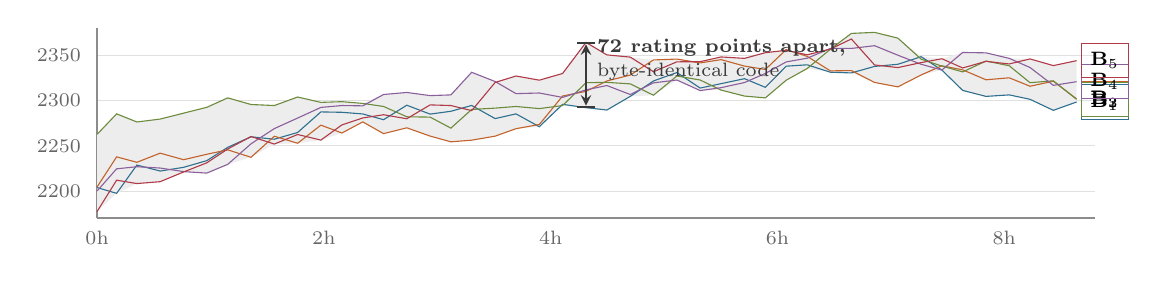
\begin{tikzpicture}[x=1cm,y=1cm,line width=0.4pt]
\draw[gridline] (0.000,0.344) -- (12.672,0.344);
\node[axlab,anchor=east] at (-0.080,0.344) {2200};
\draw[gridline] (0.000,0.918) -- (12.672,0.918);
\node[axlab,anchor=east] at (-0.080,0.918) {2250};
\draw[gridline] (0.000,1.492) -- (12.672,1.492);
\node[axlab,anchor=east] at (-0.080,1.492) {2300};
\draw[gridline] (0.000,2.066) -- (12.672,2.066);
\node[axlab,anchor=east] at (-0.080,2.066) {2350};
\node[axlab,anchor=north] at (0.000,-0.043) {0h};
\node[axlab,anchor=north] at (2.880,-0.043) {2h};
\node[axlab,anchor=north] at (5.760,-0.043) {4h};
\node[axlab,anchor=north] at (8.640,-0.043) {6h};
\node[axlab,anchor=north] at (11.520,-0.043) {8h};
\draw[axline] (0.000,0.000) -- (12.672,0.000);
\draw[axline] (0.000,0.000) -- (0.000,2.410);
\fill[band] (0.000,1.064) -- (0.248,1.324) -- (0.505,1.221) -- (0.801,1.258) -- (1.098,1.333) -- (1.393,1.407) -- (1.659,1.527) -- (1.955,1.443) -- (2.251,1.430) -- (2.547,1.538) -- (2.842,1.470) -- (3.109,1.479) -- (3.374,1.457) -- (3.638,1.570) -- (3.933,1.596) -- (4.229,1.556) -- (4.493,1.565) -- (4.757,1.852) -- (5.055,1.735) -- (5.320,1.805) -- (5.616,1.752) -- (5.912,1.837) -- (6.209,2.232) -- (6.474,2.073) -- (6.771,2.045) -- (7.066,2.009) -- (7.363,2.020) -- (7.659,1.987) -- (7.925,2.047) -- (8.222,2.029) -- (8.487,2.101) -- (8.752,2.141) -- (9.018,2.074) -- (9.313,2.155) -- (9.579,2.346) -- (9.874,2.359) -- (10.170,2.286) -- (10.465,2.050) -- (10.729,2.024) -- (10.993,2.104) -- (11.289,2.099) -- (11.584,2.029) -- (11.848,2.022) -- (12.144,1.937) -- (12.440,2.000) -- (12.440,1.475) -- (12.144,1.369) -- (11.848,1.509) -- (11.584,1.565) -- (11.289,1.546) -- (10.993,1.622) -- (10.729,1.880) -- (10.465,1.818) -- (10.170,1.667) -- (9.874,1.723) -- (9.579,1.844) -- (9.313,1.853) -- (9.018,1.900) -- (8.752,1.752) -- (8.487,1.527) -- (8.222,1.550) -- (7.925,1.626) -- (7.659,1.620) -- (7.363,1.754) -- (7.066,1.561) -- (6.771,1.546) -- (6.474,1.373) -- (6.209,1.403) -- (5.912,1.430) -- (5.616,1.161) -- (5.320,1.136) -- (5.055,1.041) -- (4.757,0.990) -- (4.493,0.969) -- (4.229,1.042) -- (3.933,1.147) -- (3.638,1.073) -- (3.374,1.222) -- (3.109,1.081) -- (2.842,0.991) -- (2.547,0.951) -- (2.251,0.941) -- (1.955,0.773) -- (1.659,0.683) -- (1.393,0.572) -- (1.098,0.586) -- (0.801,0.463) -- (0.505,0.439) -- (0.248,0.315) -- (0.000,0.084) -- cycle;
\draw[c1] (0.000,0.388) -- (0.248,0.315) -- (0.505,0.674) -- (0.801,0.598) -- (1.098,0.645) -- (1.393,0.730) -- (1.659,0.899) -- (1.955,1.033) -- (2.251,1.002) -- (2.547,1.088) -- (2.842,1.349) -- (3.109,1.344) -- (3.374,1.323) -- (3.638,1.250) -- (3.933,1.434) -- (4.229,1.321) -- (4.493,1.357) -- (4.757,1.431) -- (5.055,1.264) -- (5.320,1.324) -- (5.616,1.161) -- (5.912,1.445) -- (6.209,1.403) -- (6.474,1.373) -- (6.771,1.546) -- (7.066,1.742) -- (7.363,1.849) -- (7.659,1.652) -- (7.925,1.708) -- (8.222,1.771) -- (8.487,1.661) -- (8.752,1.930) -- (9.018,1.947) -- (9.313,1.853) -- (9.579,1.844) -- (9.874,1.927) -- (10.170,1.954) -- (10.465,2.050) -- (10.729,1.880) -- (10.993,1.622) -- (11.289,1.546) -- (11.584,1.565) -- (11.848,1.509) -- (12.144,1.369) -- (12.440,1.475);
\node[ptlab,c1,anchor=west] at (12.490,1.475) {B$_1$};
\draw[c2] (0.000,0.396) -- (0.248,0.778) -- (0.505,0.709) -- (0.801,0.825) -- (1.098,0.742) -- (1.393,0.811) -- (1.659,0.867) -- (1.955,0.773) -- (2.251,1.040) -- (2.547,0.951) -- (2.842,1.181) -- (3.109,1.081) -- (3.374,1.222) -- (3.638,1.073) -- (3.933,1.147) -- (4.229,1.042) -- (4.493,0.969) -- (4.757,0.990) -- (5.055,1.041) -- (5.320,1.136) -- (5.616,1.189) -- (5.912,1.551) -- (6.209,1.610) -- (6.474,1.742) -- (6.771,1.817) -- (7.066,2.009) -- (7.363,2.020) -- (7.659,1.971) -- (7.925,2.013) -- (8.222,1.931) -- (8.487,1.888) -- (8.752,2.141) -- (9.018,2.054) -- (9.313,1.870) -- (9.579,1.874) -- (9.874,1.723) -- (10.170,1.667) -- (10.465,1.818) -- (10.729,1.935) -- (10.993,1.883) -- (11.289,1.757) -- (11.584,1.782) -- (11.848,1.675) -- (12.144,1.739) -- (12.440,1.513);
\node[ptlab,c2,anchor=west] at (12.490,1.513) {B$_2$};
\draw[c3] (0.000,1.064) -- (0.248,1.324) -- (0.505,1.221) -- (0.801,1.258) -- (1.098,1.333) -- (1.393,1.407) -- (1.659,1.527) -- (1.955,1.443) -- (2.251,1.430) -- (2.547,1.538) -- (2.842,1.470) -- (3.109,1.479) -- (3.374,1.457) -- (3.638,1.418) -- (3.933,1.287) -- (4.229,1.283) -- (4.493,1.143) -- (4.757,1.380) -- (5.055,1.397) -- (5.320,1.418) -- (5.616,1.391) -- (5.912,1.430) -- (6.209,1.720) -- (6.474,1.724) -- (6.771,1.705) -- (7.066,1.561) -- (7.363,1.805) -- (7.659,1.754) -- (7.925,1.626) -- (8.222,1.550) -- (8.487,1.527) -- (8.752,1.752) -- (9.018,1.900) -- (9.313,2.145) -- (9.579,2.346) -- (9.874,2.359) -- (10.170,2.286) -- (10.465,2.019) -- (10.729,1.931) -- (10.993,1.857) -- (11.289,1.995) -- (11.584,1.935) -- (11.848,1.720) -- (12.144,1.744) -- (12.440,1.509);
\node[ptlab,c3,anchor=west] at (12.490,1.509) {B$_3$};
\draw[c4] (0.000,0.345) -- (0.248,0.626) -- (0.505,0.653) -- (0.801,0.636) -- (1.098,0.591) -- (1.393,0.572) -- (1.659,0.683) -- (1.955,0.944) -- (2.251,1.137) -- (2.547,1.271) -- (2.842,1.406) -- (3.109,1.430) -- (3.374,1.426) -- (3.638,1.570) -- (3.933,1.596) -- (4.229,1.556) -- (4.493,1.565) -- (4.757,1.852) -- (5.055,1.735) -- (5.320,1.581) -- (5.616,1.589) -- (5.912,1.533) -- (6.209,1.629) -- (6.474,1.684) -- (6.771,1.570) -- (7.066,1.718) -- (7.363,1.754) -- (7.659,1.620) -- (7.925,1.657) -- (8.222,1.722) -- (8.487,1.838) -- (8.752,1.984) -- (9.018,2.031) -- (9.313,2.155) -- (9.579,2.155) -- (9.874,2.190) -- (10.170,2.069) -- (10.465,1.954) -- (10.729,1.881) -- (10.993,2.104) -- (11.289,2.099) -- (11.584,2.029) -- (11.848,1.913) -- (12.144,1.686) -- (12.440,1.733);
\node[ptlab,c4,anchor=west] at (12.490,1.733) {B$_4$};
\draw[c5] (0.000,0.084) -- (0.248,0.482) -- (0.505,0.439) -- (0.801,0.463) -- (1.098,0.586) -- (1.393,0.702) -- (1.659,0.878) -- (1.955,1.036) -- (2.251,0.941) -- (2.547,1.062) -- (2.842,0.991) -- (3.109,1.184) -- (3.374,1.272) -- (3.638,1.313) -- (3.933,1.262) -- (4.229,1.438) -- (4.493,1.430) -- (4.757,1.365) -- (5.055,1.723) -- (5.320,1.805) -- (5.616,1.752) -- (5.912,1.837) -- (6.209,2.232) -- (6.474,2.073) -- (6.771,2.045) -- (7.066,1.859) -- (7.363,1.985) -- (7.659,1.987) -- (7.925,2.047) -- (8.222,2.029) -- (8.487,2.101) -- (8.752,2.131) -- (9.018,2.074) -- (9.313,2.147) -- (9.579,2.275) -- (9.874,1.945) -- (10.170,1.912) -- (10.465,1.975) -- (10.729,2.024) -- (10.993,1.907) -- (11.289,1.991) -- (11.584,1.958) -- (11.848,2.022) -- (12.144,1.937) -- (12.440,2.000);
\node[ptlab,c5,anchor=west] at (12.490,2.000) {B$_5$};
\draw[spreadarrow] (6.209,1.403) -- (6.209,2.232);
\node[note,anchor=south west] at (6.309,2.011) {\textbf{72 rating points apart,}};
\node[note,anchor=north west] at (6.309,2.011) {byte-identical code};
\end{tikzpicture}

\caption{\tbf{Five byte-identical builds, 8.6\,h, 45 simultaneous polls,
${\approx}3{,}000$ games each.} Band = min--max envelope per poll (mean spread
48.1, max 88.0). Per family the same builds spread 136.8 / 161.8 / 109.8 points
on average and 292.9 at peak, while their \emph{behaviour} differed by
${\le}0.010$ of the pot.}
\label{fig:noise}
\end{figure}

\begin{table}[H]
\centering\small
\caption{Fleet volume, 12--30 August 2026, recovered from the local turn logs.
Only the account's best slot is ranked, which is what makes the other four
available as simultaneous controls.}
\label{tab:volume}
\begin{tabular}{@{}lrlr@{}}
\toprule
Family & unique games & Fleet total & \\
\midrule
Bargaining  & 89{,}641 & logged turns         & 3{,}114{,}356 \\
Negotiation & 76{,}490 & unique games         & 264{,}432 \\
Persuasion  & 98{,}301 & reconstructable runs & 49 \\
\bottomrule
\end{tabular}
\end{table}

\begin{table}[H]
\centering\small
\caption{Break-even recovery (technique C) over 7{,}104 known-horizon and
31{,}208 open-horizon bargaining games. The whole bargaining deficit is one
cell, and it is the accept side: replaying the shipped decision rule over
26{,}773 logged decision points (98.79\% control fidelity) shows the stonewall
term setting the bar as low as 0.118, so it signs 0.30--0.50 offers in the
opening rounds.}
\label{tab:breakeven}
\begin{tabular}{@{}llrrrl@{}}
\toprule
Horizon & Seat & I bank & Field median & Gap & Diagnosis \\
\midrule
open     & $p_1$ & 0.530 & 0.476 & $+0.054$ & healthy \\
open     & $p_2$ & 0.501 & 0.463 & $+0.038$ & healthy \\
known 12 & $p_1$ & 0.435 & \tbf{0.816} & $\mathbf{-0.381}$ & accept bar collapses to 0.118 \\
known 12 & $p_2$ & 0.687 & 0.449 & $+0.239$ & healthy \\
\bottomrule
\end{tabular}
\end{table}

\begin{table}[H]
\centering\small
\caption{Open-horizon bargaining: the field median is approximately Rubinstein
SPE, and I sit under it in every player-1 cell (technique C, 38{,}312 games).
The exception is $\delta_{\text{us}}{=}\delta_{\text{them}}{=}0.95$, where SPE
is 0.513 but the field median is only 0.475, so demanding SPE there buys
no-deals, which is why the shipped floor targets the measured field median
rather than the equilibrium.}
\label{tab:spe}
\begin{tabular}{@{}rrrrrr@{}}
\toprule
$\delta_{\text{us}}$ & $\delta_{\text{them}}$ & mine & field median & SPE & gap \\
\midrule
0.95 & 0.80 & 0.712 & 0.825 & 0.833 & $-0.11$ \\
0.95 & 0.90 & 0.536 & 0.625 & 0.690 & $-0.09$ \\
0.90 & 0.80 & 0.595 & 0.675 & 0.714 & $-0.08$ \\
0.90 & 0.90 & 0.449 & 0.525 & 0.526 & $-0.08$ \\
1.00 & 0.90 & 0.692 & 0.775 & 1.000 & $-0.08$ \\
0.80 & 0.80 & 0.477 & 0.525 & 0.556 & $-0.05$ \\
\bottomrule
\end{tabular}
\end{table}

\begin{table}[H]
\centering\small
\caption{Five of the six changes that replicated. Each removed a \emph{strictly
dominated} choice, an option plainly worse than an available alternative with no
trade-off to price. Nothing else did.}
\label{tab:ledger}
\begin{tabular}{@{}p{0.26\linewidth}p{0.70\linewidth}@{}}
\toprule
Change & Evidence \\
\midrule
Complete-info ultimatum & I was asking 0.650 of a \emph{known} surplus on the one round they cannot refuse; 0.99 was signable. $+3.42\sigma$, $n{=}214$ \\
Rung-aware pricing & Price at the recovered valuation rungs, not guesses. $+3.9/{+}4.1\sigma$, replicated \\
Free-clock accept floor & At $\delta{=}1$ refusing is costless. ${+}0.0458$ of pot, $n{=}108$, $7.7\sigma$, none worse \\
Open-horizon cap collapse & The server zeroes both sides and never says so. Caught 11 of 11 \$0 games \\
Negative-signal parser & 270 buys made against messages that read as refusals; \tbf{95.6\% low quality} against a 27.5\% base rate \\
\bottomrule
\end{tabular}
\end{table}

\begin{table}[H]
\centering\small
\caption{Bounded complete-information negotiation: the same seat under two
horizons, over 10{,}740 games. Grinding to the last round is where the
family's losses are, and deal rate cannot see it, because the round-10 dump
\emph{is} a deal.}
\label{tab:endgame}
\begin{tabular}{@{}lrlr@{}}
\toprule
Cell / outcome & $n$ & banked / buyer value & rating\,/\,game \\
\midrule
$\text{max\_rounds}{=}1$, seller, complete info  & 488 & asks 0.991, signed 99.2\% & $\mathbf{+6.10}$ \\
$\text{max\_rounds}{=}10$, seller, complete info & 469 & (split below) & $\mathbf{-4.63}$ \\
\quad closed by round 8  & 66  & 0.2365 & $+5.9$ \\
\quad ground to round 10 & 403 & \tbf{0.0433} & $\mathbf{-6.4}$ \\
\bottomrule
\end{tabular}
\end{table}

\section{Extended limitations}
\label{app:lim}

Three limitations were compressed out of \S7. \tbf{(i) The persuasion buyer seat
admits no per-round counterfactual even in principle}: quality on declined rounds
is never revealed, so technique (D) answers only the aggregate question ``am I
leaking in this cell'', never ``should I have bought round~7''.
\tbf{(ii) The offline simulator is optimistic.} I built a local bargaining
engine (real rules, my seat played by the shipped code, the other seat by a
field fitted to 15{,}788 real games plus eight adversarial archetypes). It
reproduces per-cell median settlement rounds but scores ${\approx}{+}0.03$ of pot
high, with a ${\pm}45$-rating noise floor per world at $n{=}4{,}000$, so I used
it only to choose which arm deserved a live window and never shipped on it
alone. \tbf{(iii) Operational failure modes cost me more than any strategy
error.} Three recur: a deploy that writes arm flags back into the repository
working tree (hit five times, and the reason 27 tests fail on my final-night
tree); an entry point outside the copied package, so sibling agents silently ran
stale code; and force-killing an agent mid-game, which abandons in-flight games
at the 5th percentile and can trip a 30-minute queue ban. Draining with a
deadline rather than a kill is the only safe stop.

\tbf{(iv) Opponent modelling is stable but unreachable where it would pay.}
\S8 reports split-half $r{=}0.786$ across the 19 opponent\,$\times$\,cell
profiles with ${\ge}25$ purchases in both halves, which is real but is also the
whole usable sample. Three things block the rest. Identity is withheld in
49.9\% of games; the named half spreads 16{,}498 games over 227 opponents and
15 cells, about five games per profile, and behaviour differs by cell so they
cannot be pooled; and quality is redacted on every round I passed (0 of 42{,}616
unbought rounds ever showed it), so a reputation table has \emph{zero} entries
in precisely the cells where I buy nothing and most need one. That is why the
shipped buyer reads the seller's rationing rate within the current game, which
is visible whether or not I buy, instead of a cross-game profile.

\section{A note on the Simpson's paradox I nearly shipped on}
\label{app:simpson}

A late candidate rule, ``take a recommendation only from a seller who has
already spent a sale to decline one'', looked refuted when pooled across all
fifteen $(m,p)$ cells: subsequent dud rates of 0.285 / 0.287 / 0.286 / 0.315
for sellers who had declined 0 / 1 / 2 / 3--4 of their first four rounds. Split
by cell it reverses and becomes monotone: inside $(m{=}1.20, p{=}0.80)$,
$n{=}9{,}932$, the same buckets read 0.160 / 0.102 / 0.081 / \tbf{0.069}
against a break-even of $1-1/m = 0.167$. The pooled number is dominated by easy
cells where everyone buys everything regardless. I did not ship it, for the
reason the rest of this paper argues: at 2.2\% of my games it was worth
${\approx}{+}2.6$ rating points, far below what the remaining window could
measure, and a fourth simultaneous change would have destroyed my ability to
read the three already running.

\section{Three properties of the scoring rule}
\label{app:scoring}

\tbf{The aggregate rewards balance, and I optimised the wrong object for two
weeks.} Overall rank is the \emph{unweighted mean} of the three family ratings,
and only an account's best slot is ranked. Judged per family, negotiation was my
best return per game; judged per \emph{overall} point it was nearly worthless,
because ${+}300$ more negotiation is ${+}100$ overall and hard, while ${+}180$ in
each weak family is ${+}120$ and was what the arms already targeted. At the time
I noticed, I sat 11th at 2301.5 with negotiation 2875 (4th best on the board) and
bargaining 2021; the 4th-placed account held that same bargaining rating.
\tbf{Nobody in the top ten was balanced}, which is the strongest structural
incentive the scoring rule creates and the one I was slowest to see.

\tbf{The reference pool defends itself against sabotage.} A natural worry is
that spare agent slots could be spent depressing rivals' ratings. Besides being
prohibited and trivially detectable, it is self-defeating on the mechanism:
percentile is scored against payoffs earned on the same configuration, and
competition games join that pool as they are played, so every no-deal forced on
an opponent injects a bottom-of-distribution payoff that \emph{raises} the
percentile of every normal payoff scored afterwards. Attacking the field inflates
it. There is also no opponent selection anywhere in the API, so the damage would
spray uniformly across the 227 opponents I faced.

\tbf{The underlying data will come from the organisers rather than from me.}
Every number here is computed from my own turn logs, which also carry the
transcripts of the agents I was matched against, and those are not released
alongside the code. The organisers have said they will publish the full game
record for every agent, which supersedes anything I could have attached: it
covers the whole field rather than one account, and it comes from the party that
ran the games. The analysis scripts are released now, so the method can be
audited ahead of the data it will run on.

\tbf{The garden of forking paths is wide here.} One persuasion arm, analysed
three defensible ways on the same data, read $-3.11\sigma$ across 3 cells,
$-0.82\sigma$ across 33, and $+3.02\sigma$ across 44, depending only on the
inclusion threshold for how many games a configuration needed to enter the
sample. Pre-registering the cell filter before looking is not optional at this
noise level.

\end{document}
